\chapter{User Manual}\label{cap:evaluation}
\section{Graphical overview of RealityEnhance}
We will now go through some of the application's graphical user interfaces. This should give a summary of the fundamental flows present in the program and accommodate the user with regard to the interface.
\pagebreak

\subsection{App start page}
The fisrt thing any user will see when they lounch the app on their phone is the loading page. This page is a simple loading screen that will be displayed while the app is loading. In the loading phase the app will check if the user is able to run the app on their phone and if the phone has the necessary sensors to run the app. If the user is able to run the app, the app will load the main page. If the user is not able to run the app, the app will display a message that the user is not able to run the app on their phone.
\begin{figure}[h!]
    \begin{center}
        
\includegraphics[scale=0.5]{img/App_mock/iPhone 14 - 1.png}
        \caption{Loading page}
        \label{fig:loading-page}
    \end{center}
\end{figure}
\pagebreak


\subsection{App burger button}
The burger button is a button that is present on every page of the app. It is used to open the side menu. The side menu is used to navigate through the app. In the burger button we have access to the following options: QR scanner, Library, and EXIT.
The QR scanner is used to scan a QR code and load a 3D model and a guide into the user's smartphone. The Library is used to display all the 3D models that the user has scanned. The EXIT button is used to exit the app.
\begin{figure}[h!]
    \begin{center}
        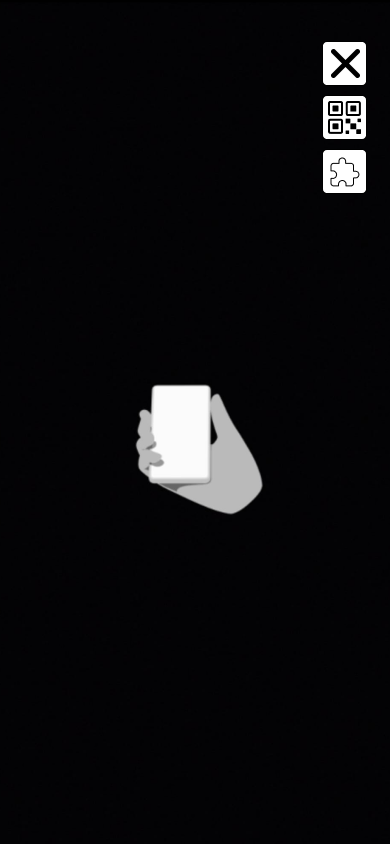
\includegraphics[scale=0.5]{img/App_mock/iPhone 14 - 2.png}
        \caption{Burger button menu}
        \label{fig:burger-button}
    \end{center}
\end{figure}
\pagebreak

\subsection{QR scanner}
In this mode, on the user's screen will be displayed a camera view. The user will have to scan a QR code. The QR code will contain a link to a 3D model and a guide. The app will download the 3D model and the guide and will display them on the user's screen. The model loaded from the QR code will be ready to use without the need to enter the Library menu. The guide will be displayed on the user's screen and the user will have to follow the guide to assemble the 3D model.

\begin{figure}[h!]
    \begin{center}
        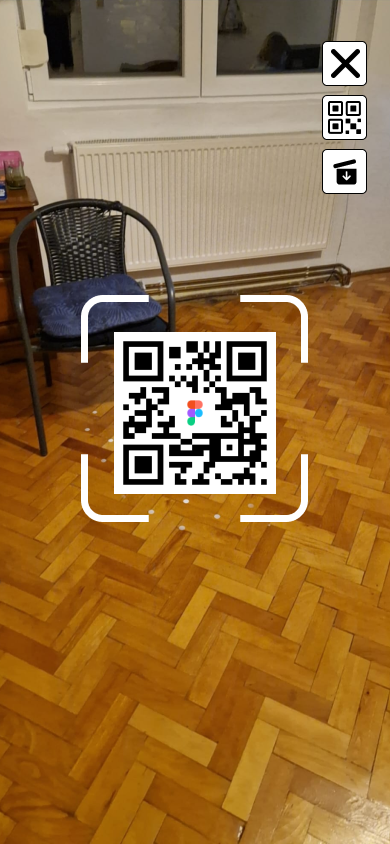
\includegraphics[scale=0.5]{img/App_mock/iPhone 14 - 3.png}
        \caption{QR scanner interface}
        \label{fig:qr-scanner}
    \end{center}
\end{figure}
\pagebreak

\subsection{QR valdiation}
If the QR code is valid, the app will display a message that the QR code is valid and will load the 3D model and the guide. If the QR code is not valid, the app will display a message that the QR code is not valid.

\begin{figure}[h!]
    \begin{center}
        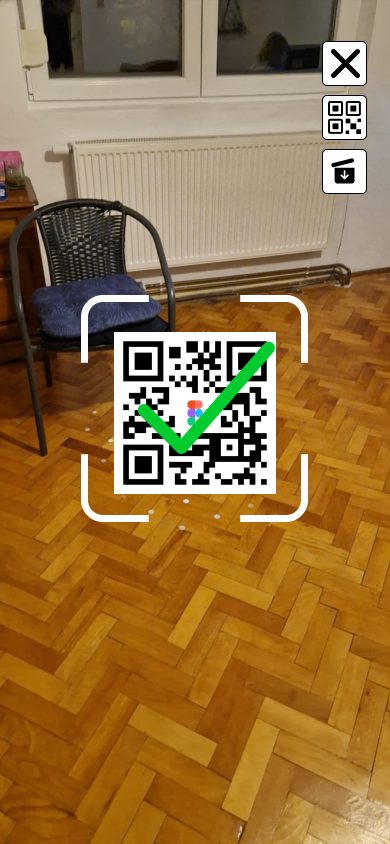
\includegraphics[scale=0.5]{img/App_mock/iPhone 14 - 4.png}
        \caption{QR code is valid}
        \label{fig:qr-valdiation}
    \end{center}
\end{figure}
\pagebreak

\subsection{AR vision}
After a model is loaded, the AR moduls will use the phone's camera to find out what is around the user. It will make a 3D model of the environment and will place the 3D model on top of the environment. The user will have a guide of the app is understanding the surroundings (a mesh of the planes will be displayed on the screen).
\begin{figure}[h!]
    \begin{center}
        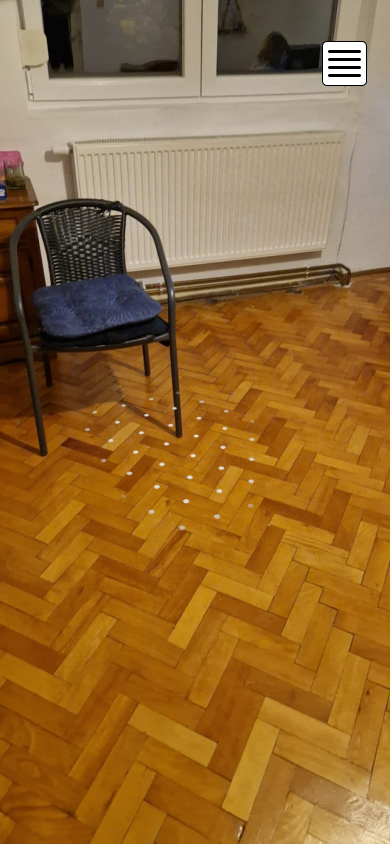
\includegraphics[scale=0.5]{img/App_mock/iPhone 14 - 5.png}
        \caption{AR vision interface}
        \label{fig:ar-vision}
    \end{center}
\end{figure}

\pagebreak

\subsection{Adding a model}
After the app has a basic understanding of the surroundings and a model loaded, the user can click on the screen to add an object to the scene. This object will be placed on the screen and the user will be able to move it around the screen. The user will be able to move the object around the screen by press-and-hold the object and moving phone around or draging the object with his/her finger across the screen. The user will be able to rotate the object by rotating the model using two fingers (like opening a bottlle cap(rotating clock-wised) or closing a bottlle cap(rotating counter-clock-wised)). The user will be able to scale the object by pinching the screen. The user is not bound to use just a single object. The user can add multiple objects to the scene and move them around the screen. The user will be able to add another object by clicking on the screen in a place where an object is not present.
\begin{figure}[!h]
    \begin{center}
        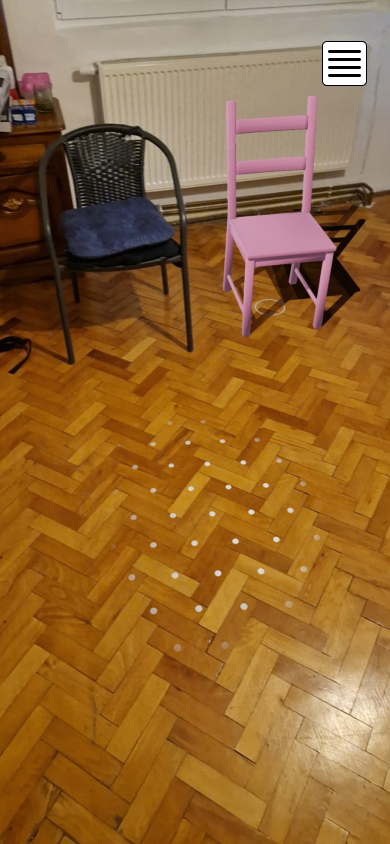
\includegraphics[scale=0.5]{img/App_mock/iPhone 14 - 6.png}
        \caption{Adding a model}
        \label{fig:add-a-model}
    \end{center}
\end{figure}
\pagebreak

\subsection{Removing a model}
The user will be able to remove the object by clicking and holding on the object and then clicking on the remove button. The user will be able to remove multiple objects at the same time by clicking on the reset all button.
\begin{figure}[h!]
    \begin{center}
        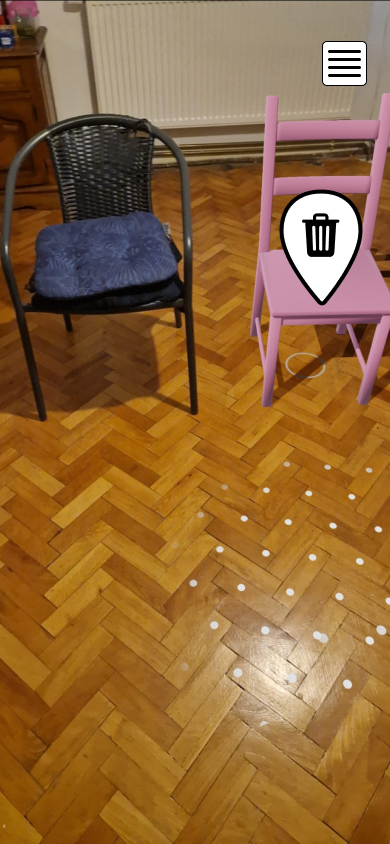
\includegraphics[scale=0.5]{img/App_mock/iPhone 14 - 7.png}
        \caption{Removing a model}
        \label{fig:remove-a-model}
    \end{center}
\end{figure}
\pagebreak


\begin{center}
    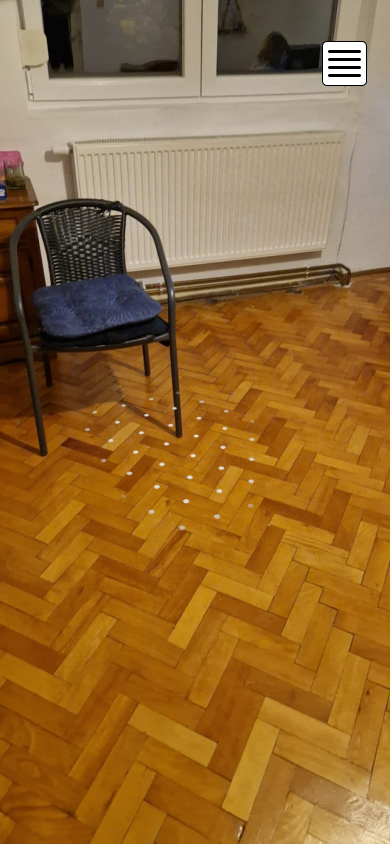
\includegraphics[scale=0.5]{img/App_mock/iPhone 14 - 8.png}
\end{center}
\pagebreak

\begin{center}
    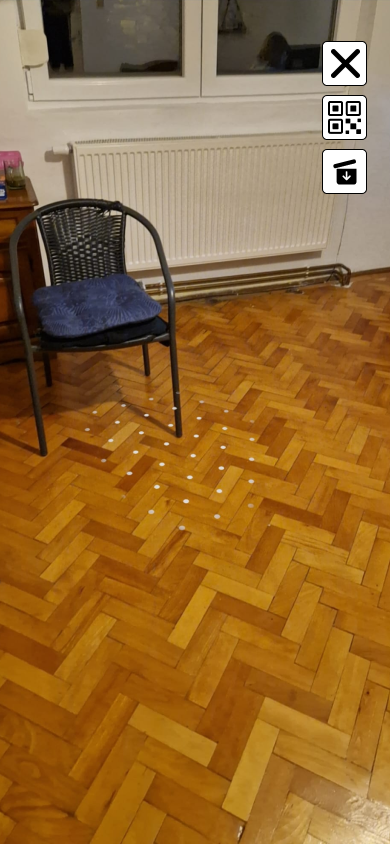
\includegraphics[scale=0.5]{img/App_mock/iPhone 14 - 9.png}
\end{center}
\pagebreak

\subsection{Library}
When the user clicks on the Library button in the burger menu, the app will display the Library interface. The Library interface will display all the 3D models that the user has scanned. The user will be able to select a model and load it into the AR vision mode. In the Library interface, the user can search for a model and add a model to the Library. The user can also delete a model from the Library.
\begin{figure}[h!]
    \begin{center}
        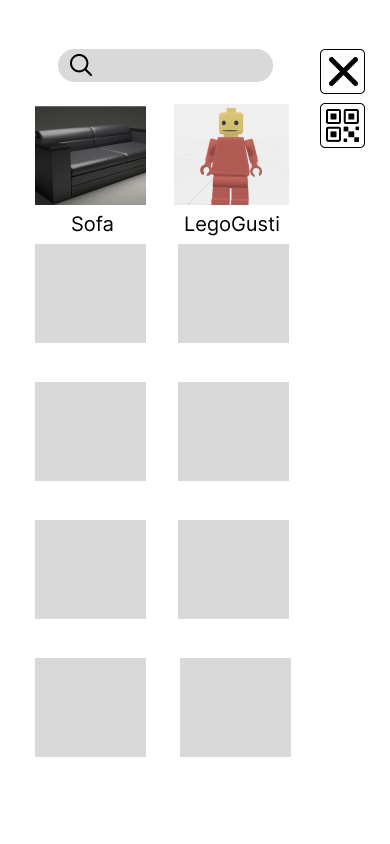
\includegraphics[scale=0.5]{img/App_mock/iPhone 14 - 10.png}
        \caption{Library interface}
        \label{fig:library}
    \end{center}
\end{figure}
\pagebreak

\subsection{Using multiple models at the same time}
The user will be able to use multiple models at the same time. The user will be able to add multiple models to the scene and move them around the screen. The user will be able to add another model by clicking on the screen in a place where an object is not present. The guide for assembling or building a model will be displayed on the screen when in the scene is present just one object.
\begin{figure}[h!]
    \begin{center}
        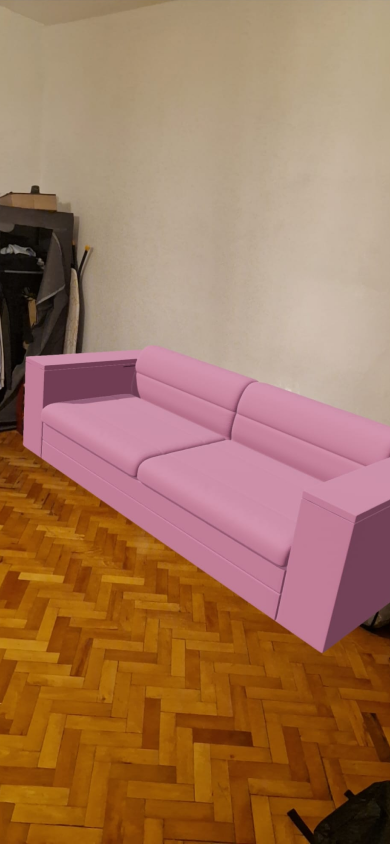
\includegraphics[scale=0.5]{img/App_mock/iPhone 14 - 11.png}
        \caption{Using multiple models}
        \label{fig:using-multiple-models}
    \end{center}
\end{figure}
\pagebreak

\section{Proof of concept}

\section{Domains of application}
\subsection{Interior designing}
\subsection{Outdoor designing}
\subsection{3D printing}
\subsection{Architecture}
\subsection{Pedagogical instrument}
